\section{Control de Formaciones en Sistemas No Holonómicos }
\subsection{Estructura Virtual con Generador de Trayectorias}

Como en la capa maestra de Siwek~\cite{siwek2024consensus}, un generador de trayectorias mueve la estructura virtual y cada robot rastrea su lugar dentro de ella:

\begin{center}
\ifshow
    \animategraphics[autoplay,loop,height=3.8cm]{10}{Pics/vs_frames/vs-}{0}{743}
\else
    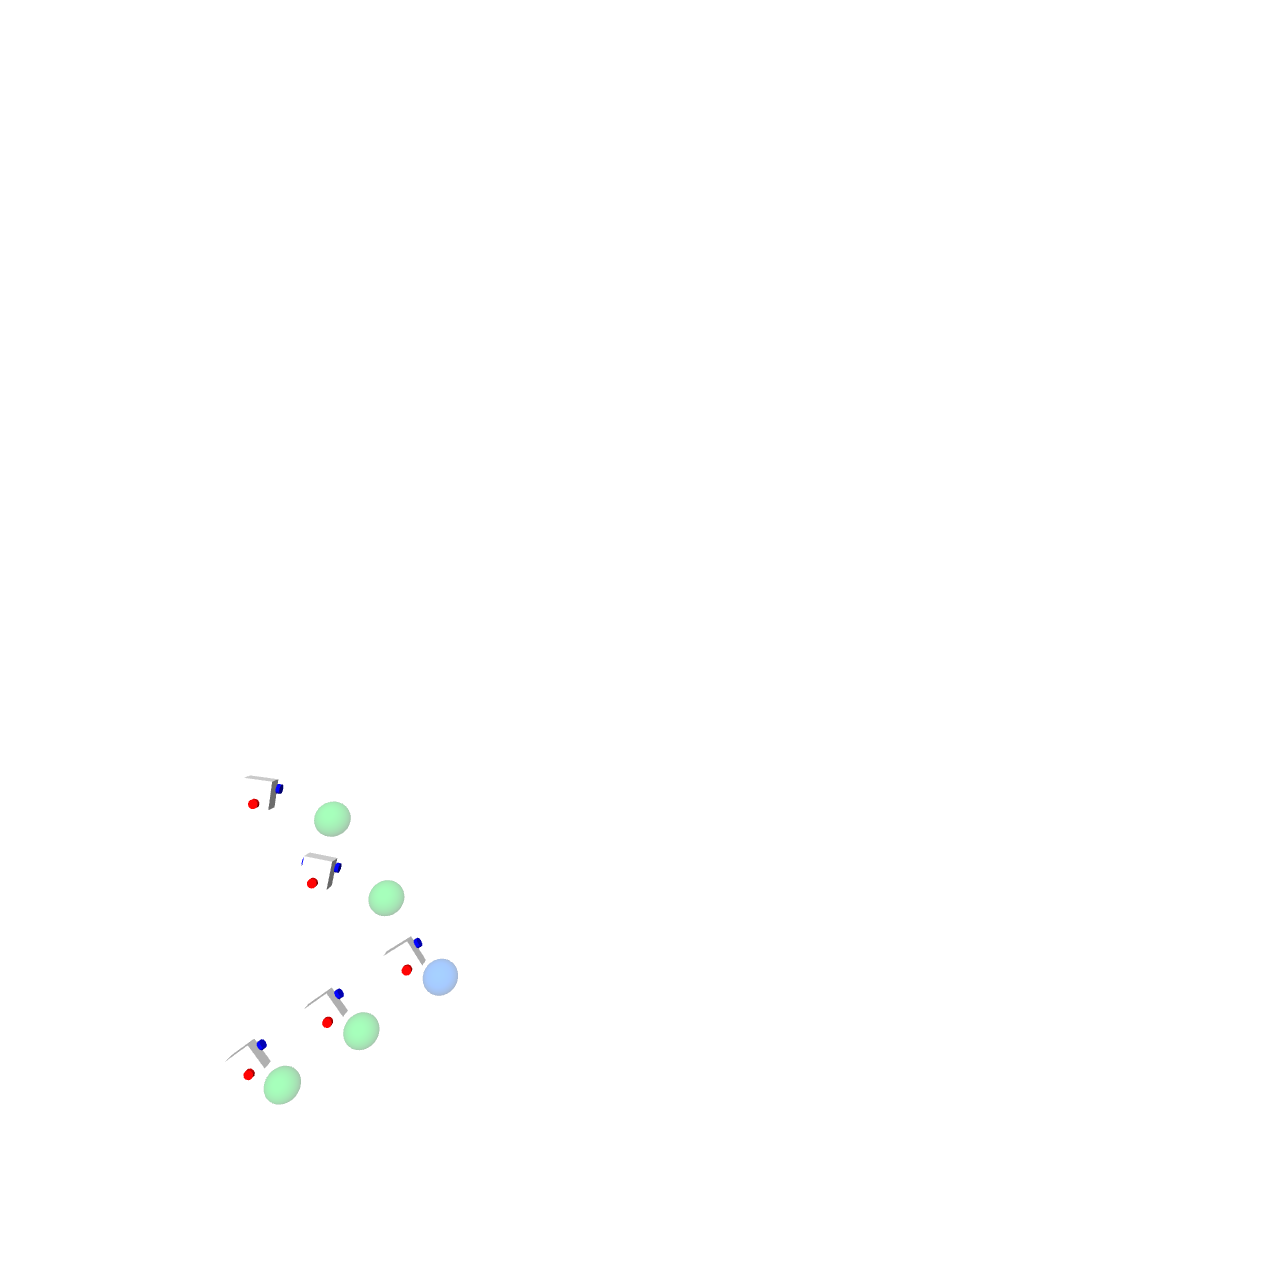
\includegraphics[height=3.8cm]{Pics/vs_frames/vs-370.png}
\fi
\end{center}
\begin{center}
\footnotesize Simulación en Gazebo de la estructura virtual siguiendo su trayectoria
\end{center}
